\begin{frame}
    \frametitle{Audioverarbeitung}
    \framesubtitle{Spektrogramm}
    Visualisierung von Signalen in einem Spektrogramm:
    \begin{itemize}
        \item Visualisiert den zeitlichen Verlauf des Frequenzspektrums
        \item Für jeden Zeitpunkt eine Fourier Analyse
        \item Signalanalyse, Musikerkennung
    \end{itemize} 
    \begin{columns}
        \begin{column}{120px}
            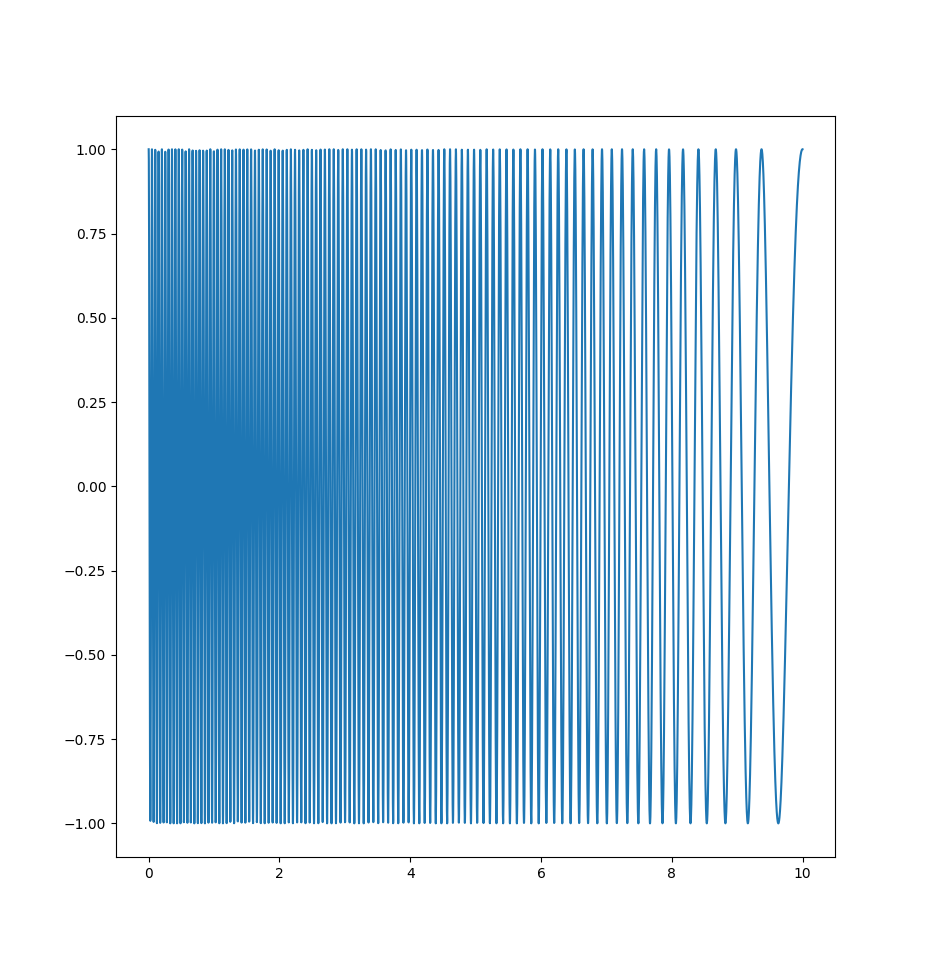
\includegraphics[width=120px]{images/04-applications-audio-chirp.png}
        \end{column}
        \hspace*{-25px}
        \begin{column}{5px}
            $\rightarrow$
        \end{column}
        \hspace*{-25px}
        \begin{column}{120px}
            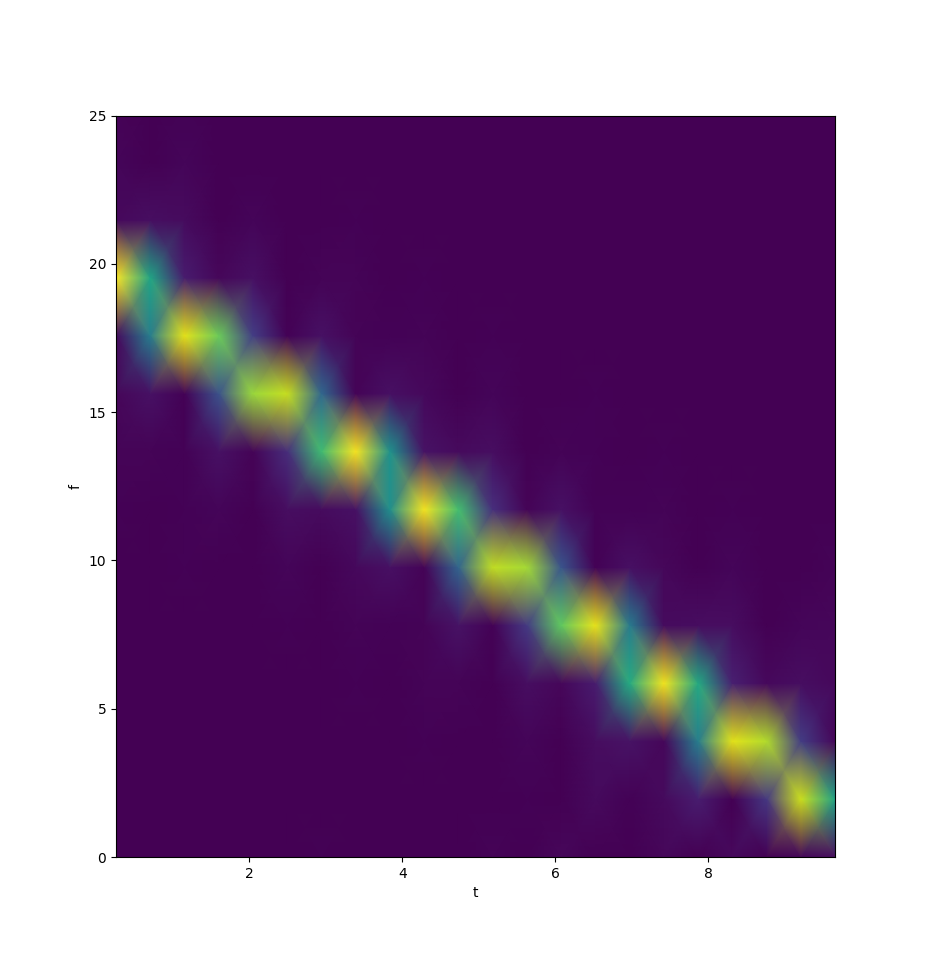
\includegraphics[width=120px]{images/04-applications-audio-chirp-spectrogram.png} 
        \end{column}
    \end{columns}
\end{frame}

\begin{frame}
    \frametitle{Audioverarbeitung}
    \framesubtitle{Frequenzfilterung}
    Filtern von Frequenzen:
    \begin{itemize}
        \item Identifizieren von Störfrequenzen
        \item Eliminierung von diesem aus Frequenzspektrum
        \item Inverse Fourier Transformation anwenden
    \end{itemize}
\end{frame}

\begin{frame}
    \frametitle{Anwendungen}
    \framesubtitle{Audio}

    \begin{columns}
        \begin{column}{160px}
            \centering
            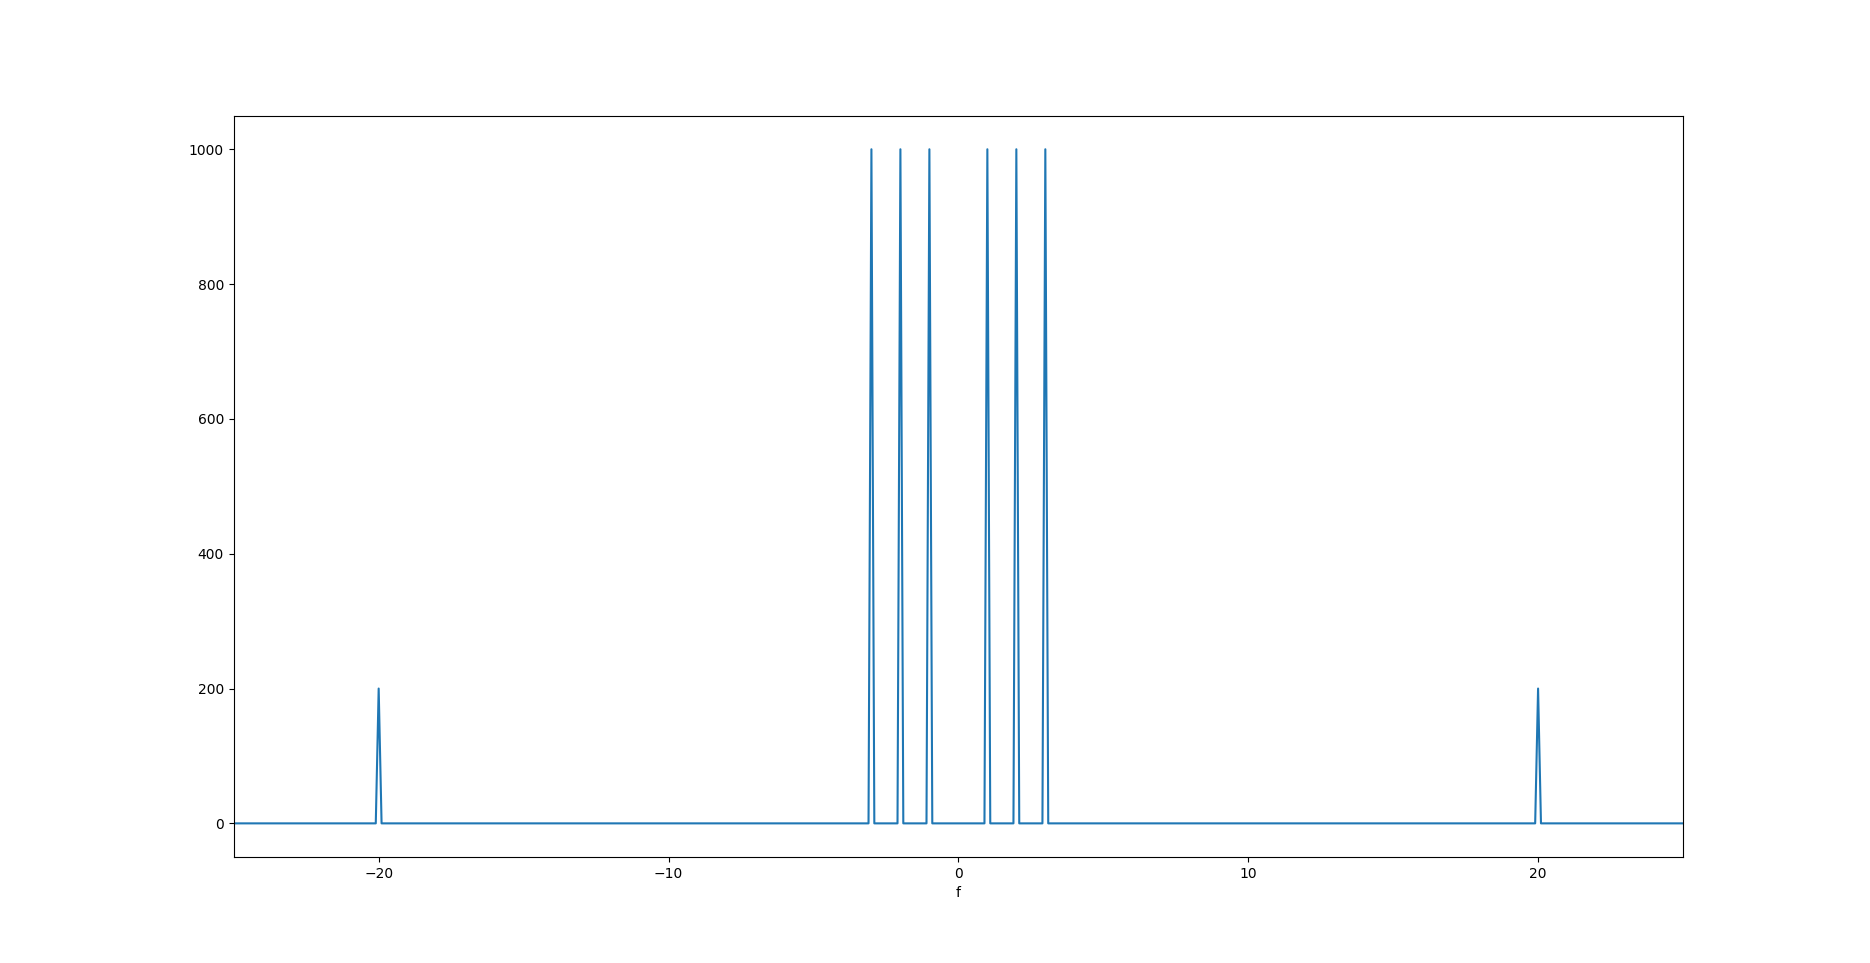
\includegraphics[width=160px]{images/04-applications-audio-noisy-signal-ft.png}
            $\downarrow$
            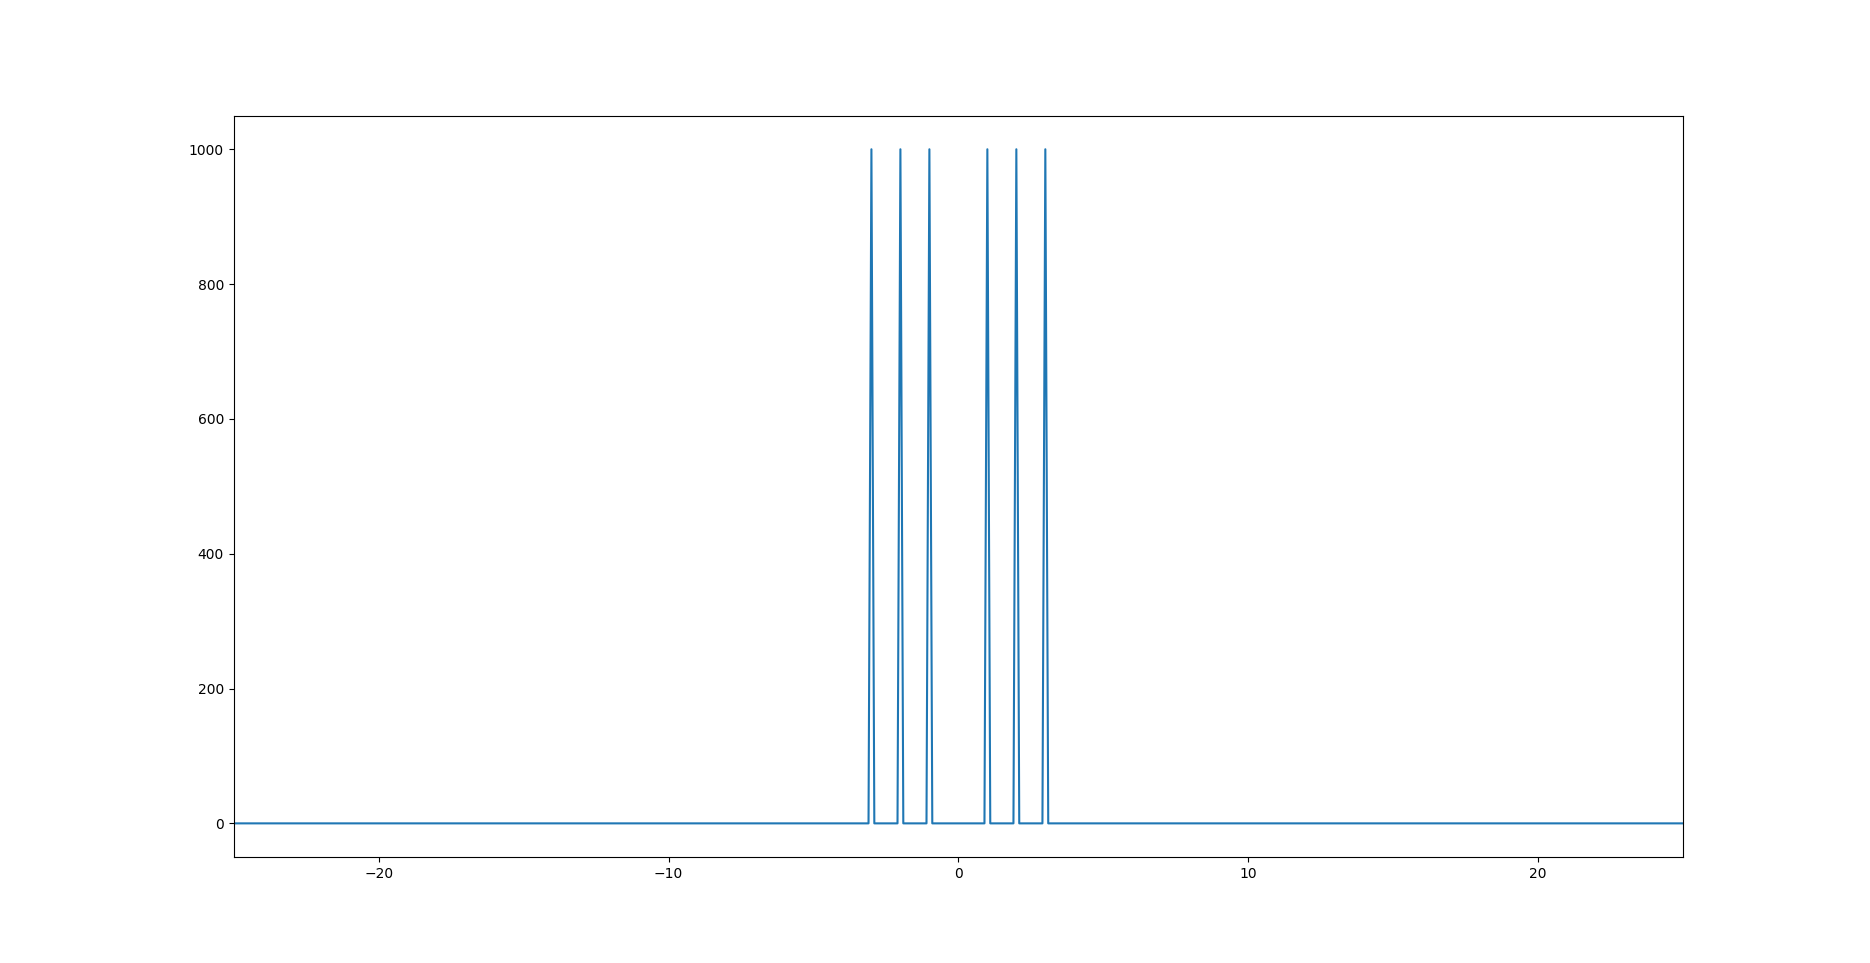
\includegraphics[width=160px]{images/04-applications-audio-clean-signal-ft.png}
        \end{column}
        \hspace*{-25px}
        \begin{column}{1px}
            \vspace*{-13px}
            \begin{align*}
                \overset{FT}\longleftarrow \\ \\ \\ \\ \\ \\
                \overset{IFT}\longrightarrow
            \end{align*}
        \end{column}
        \hspace*{-25px}
        \begin{column}{100px}
            \centering
            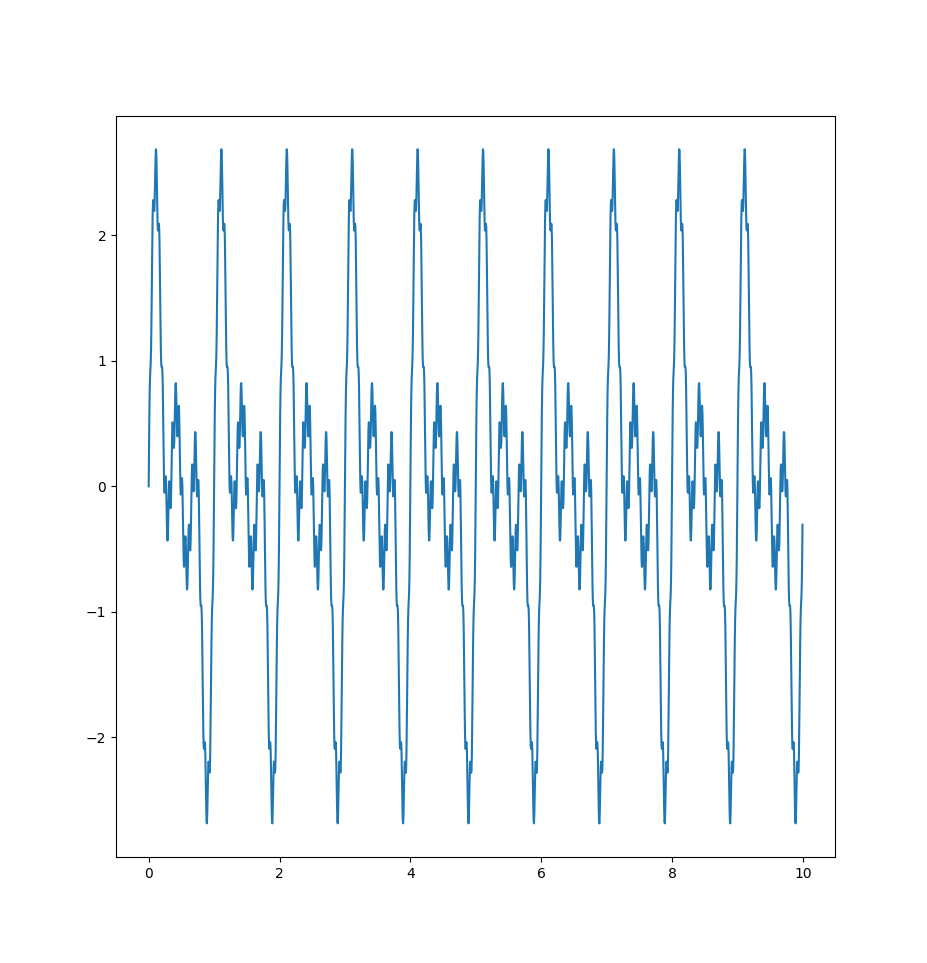
\includegraphics[width=100px]{images/04-applications-audio-noisy-signal.png}
            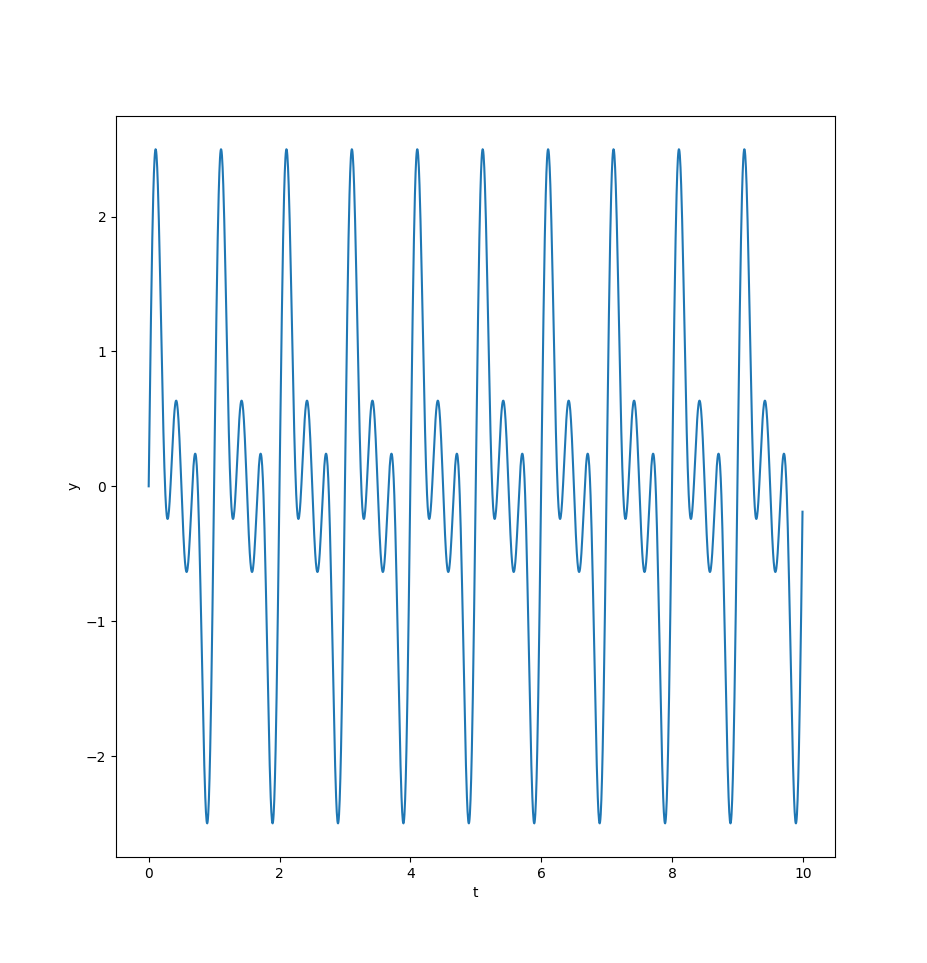
\includegraphics[width=100px]{images/04-applications-audio-clean-signal-ift.png}
        \end{column}
    \end{columns}
\end{frame}

